\documentclass[aspectratio=169,t,9pt]{beamer}
% GitHub Actions setup: PDF now built automatically, not stored in git repo
% License: MIT-Lizenz (https://opensource.org/licenses/MIT)
% Author: Bitcoin Entdecken / Bitcoin Austria

% Metropolis theme - Modern, minimalist Beamer theme
% Source: https://github.com/matze/mtheme
% License: Creative Commons Attribution-ShareAlike 4.0 International
% Features: Clean design, optional progress bar, maximizes content space
\usetheme[progressbar=foot]{metropolis}  % Enable progress bar in footer

% Bitcoin Entdecken style package
\usepackage{../styles/bitcoin-entdecken}

% Title information using Bitcoin Entdecken style helpers
\bitcointitle{Bitcoin: Häufige Missverständnisse und was wirklich dahinter steckt}{Ein faktenbasierter Impulsvortrag}
\bitcointitlegraphic{pix/missverstaendnisse.jpg}

% Include auto-generated count of misconceptions
\input{misconception-count.tex}

\begin{document}
\renewcommand{\thefootnote}{\arabic{footnote}}
\renewcommand{\thempfootnote}{\arabic{mpfootnote}}

% Title slide
\begin{frame}
	\titlepage
\end{frame}

% Table of contents
\begin{frame}{Überblick}
	\tableofcontents
\end{frame}

\begin{frame}{Warum entstehen Bitcoin-Missverständnisse?}
	\begin{itemize}
		\item \textbf{Komplexe Technologie} - Schwer verständlich für Laien
		\item \textbf{Falscher Fokus} - Die eigentlichen Fragen werden nicht gestellt
		\item \textbf{Medienverzerrung} - Sensationelle Berichterstattung
		\item \textbf{Schnelle Entwicklung} - Veraltete Informationen halten sich hartnäckig
		\item \textbf{Emotionale Diskussionen} - Fakten vs. Meinungen
		\item \textbf{Interessenskonflikte} - Verschiedene Akteure mit eigenen Agenden
	\end{itemize}
	\vspace{2em}
	\begin{alertblock}{\textcolor{white}{Ziel dieser Präsentation}}
		\vspace{3pt}
		Fakten statt Mythen - Was steht hinter den Argumenten?
		\vspace{3pt}
	\end{alertblock}
\end{frame}

\begin{frame}[plain]
	\vfill
	\begin{center}
		{\Large \textbf{Die \totalmisconceptions\ häufigsten Missverständnisse}}
		\vspace{1em}
		\roundedimage{pix/missverstaendnisse.jpg}{0.7\textwidth}{2}
	\end{center}
	\vfill
\end{frame}

\misconceptionslide[pix/mining.jpg]{Umweltauswirkungen}{Bitcoin-Mining verbraucht zu viel Energie und zerstört die Umwelt}{%
	\item Energieverbrauch \textbf{essentiell}, nicht ``sinnlos''.
	\item Nur \textbf{0,5\%} des globalen Stromverbrauchs\footnotemark
	\item \textbf{52,4\%} nachhaltige Energiequellen (Anteil steigt)\footnotemark
	\item \textbf{Kohle-Anteil} massiv gesunken (unter 9\%)\footnotemark
	\item \textbf{Überschussenergie} aus alternativen Quellen (``Energy Consumer of Last Resort'')
	\item \textbf{87\%} der Mining-Hardware wird recycelt
	\only<2->{\footnotetext[1]{Cambridge Centre for Alternative Finance}}
	\only<2->{\footnotetext[2]{Cambridge Digital Mining Industry Report 2025}}
	\only<2->{\footnotetext[3]{Naturgas hat Kohle als Hauptquelle abgelöst}}
}{Mining-Effizienz steigt kontinuierlich (24\% p.a.), Umweltimpact nimmt ab.}

\misconceptionslide[pix/nichts-intrinsisches.jpg]{Kein intrinsischer Wert}{Bitcoin hat keinen intrinsischen Wert, daher ist es wertlos}{%
	\item Bitcoin hat keine laufenden Erträge, daher nicht vergleichbar
	\item Nutzen 1: \textbf{Knappheit}: limitiert auf \textbf{21 Mio}
	\item Nutzen 2: \textbf{Zensurresistenz}
	\item Nutzen 3: \textbf{Globales Zahlungsnetzwerk} (\textbf{Portabilität und Teilbarkeit})
	\only<2->{\footnotetext[1]{Emily Stanhope und der Ökonom Charles Brandt, in ``Review of Economic Philosophy''}}
}{Es gibt keinen intrinsischen Wert! Der Wert entsteht durch gesellschaftliche Zuschreibung und kollektive Akzeptanz\footnotemark}

\misconceptionslide[pix/satoshi-breakdown-20250812_121849.jpg]{Zu teuer}{Bitcoin ist zu teuer, den kann sich niemand leisten}{%
	\item Bitcoin ist in kleinste Einheiten teilbar: \textbf{1 Satoshi}
	\item \textbf{1 Bitcoin = 100.000.000 Satoshis}
	\item Man muss keinen ganzen Bitcoin kaufen, sondern kann beliebige Mengen erwerben.
	\item Der Preis eines ganzen Bitcoins ist für die Nutzung kleiner Beträge irrelevant.
	\item Vergleichbar mit Gold: statt ganzem Goldbarren, wenige Gramm oder Unzen.
}{Jeder kann Bitcoin in beliebiger Menge erwerben, unabhängig vom Preis eines ganzen Bitcoins.}

\begin{frame}[c]{Kein Wert oder zu teuer? Was nun?}
	\begin{center}
		\begin{tikzpicture}
			\clip[rounded corners=8pt] (0,0) rectangle (0.7\textwidth,0.384\textwidth);
			\node[inner sep=0pt] at (0.35\textwidth,0.192\textwidth) {
\includegraphics[width=0.7\textwidth,keepaspectratio]{pix/wert-oder-teuer-20250812_152710.jpg}};
		\end{tikzpicture}
	\end{center}
\end{frame}

\misconceptionslide[pix/volatil.jpg]{Volatilität}{Bitcoin ist zu volatil, um als Währung oder Wertaufbewahrung zu funktionieren}{%
	\item Volatilität nimmt langfristig ab, wenn auch weniger als gedacht
	\item \textbf{Weniger volatil} als \textbf{33 S\&P 500 Aktien}
	\item Typisch für neue Asset-Klassen (\textbf{price discovery})
	\item \textbf{Institutionelle Adoption} stabilisiert
	\item Langfristiger Trend in der \textbf{logarithmierten Preiskurve} sichtbar: spätere ``Täler'' liegen höher als vorherige ``Gipfel''
}{Reifung des Marktes führt zu weniger Volatilität.}

\begin{frame}[c]{Bitcoin-Preis in logarithmischen Einheiten}
	\begin{center}
		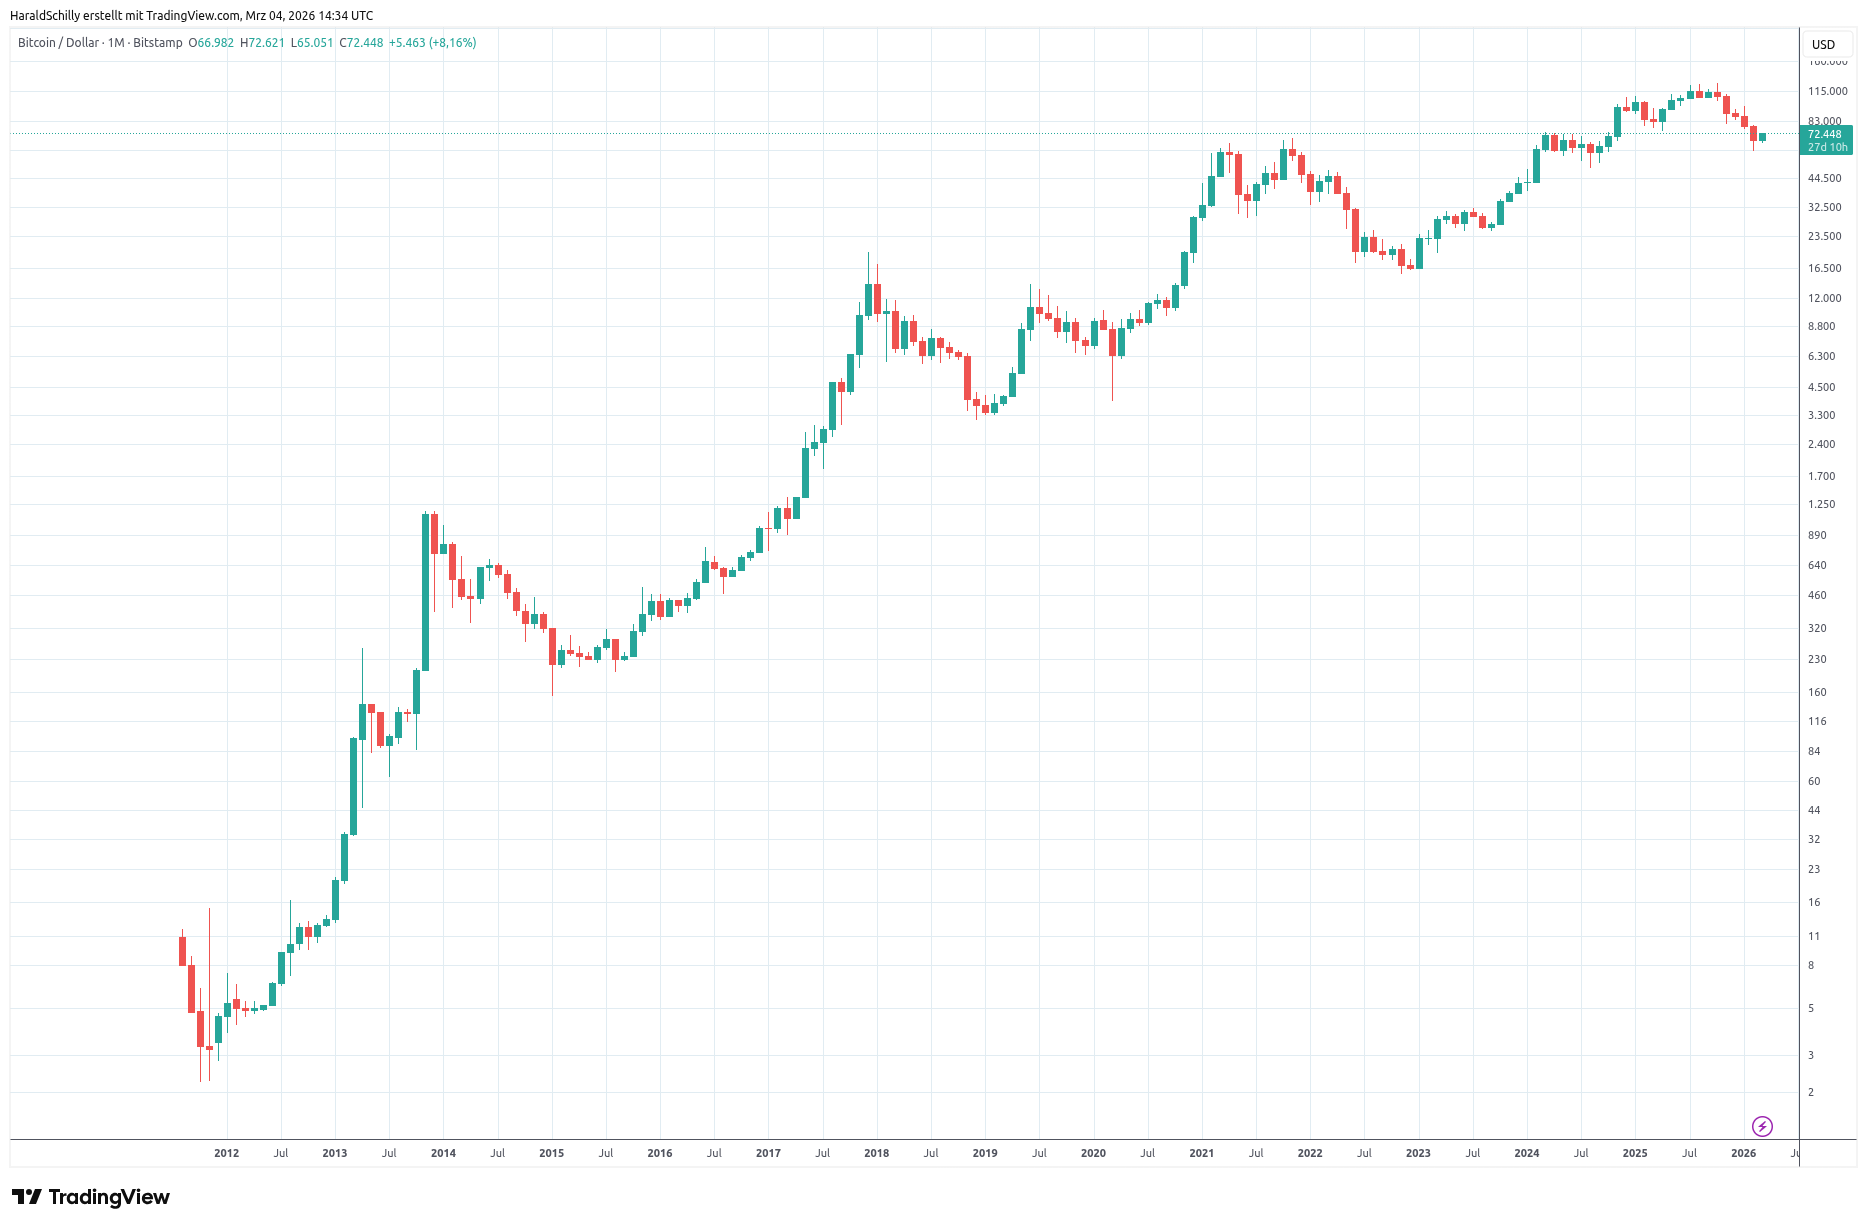
\includegraphics[width=0.9\textwidth,keepaspectratio]{pix/BTCUSD_2026-03-04_log.png}
	\end{center}
\end{frame}

\misconceptionslide[pix/verbrecher-2.jpg]{Regulierung}{Bitcoin hat keine rechtliche Grundlage und wird verboten werden}{%
	\item Legitimierung: \textbf{USA und EU} haben klare Gesetze etabliert
	\item Regulierung: betrifft die \textbf{Intermediären} (Börsen), nicht Bitcoin an sich
	\item EU: \textbf{MiCA-Verordnung} schafft seit 2025 volle Rechtssicherheit
	\item Institutionelle Compliance ist mittlerweile Industriestandard
	\item Verbote \textbf{schwer durchsetzbar} und politisch unwahrscheinlich
}{Rechtliche Klarheit ist in den meisten G20-Staaten hergestellt.}

\misconceptionslide[pix/bitcoin-skalieren-2.jpg]{Skalierbarkeit}{Bitcoin kann nur 3-4 Transaktionen pro Sekunde verarbeiten}{%
	\item \textbf{Blockchain-Trilemma}: Skalierbarkeit vs. Sicherheit vs. Dezentralisierung
	\item \textbf{Lightning Network}: bis zu \textbf{1 Million TPS} theoretisch möglich
	\item Visa: \textbf{65.000 TPS}, ca. \textbf{15-18 Bio. USD} Jahresvolumen\footnotemark
	\item Volumen: Bitcoin \textbf{$>$~25 Bio. USD} (On-Chain + Layer 2)\footnotemark
	\only<2->{\footnotetext[1]{Visa Inc. Annual Report 2024}}
	\only<2->{\footnotetext[2]{Sygnum Bank Future Finance Report, 2025}}
	\item Lightning ist global, dezentral und ohne Intermediäre
	\item VISA ist kein \textbf{Schuldverhältnis}, kein \textbf{finales Settlement} wie Bitcoin
}{Bitcoin übertrifft Visa im jährlichen Transaktionsvolumen bereits deutlich.}

\misconceptionslide[pix/blase.jpg]{Spekulationsblase}{Bitcoin ist eine Spekulationsblase}{%
	\item Blasen sind kurzfristig, über Monate, nicht über \textbf{10 Jahre}
	\item Bitcoin hatte -- wenn überhaupt -- \textbf{mehrere Blasen}
	\item Wertspeicher für langfristiges Sparen
	\item \textbf{Netzwerkeffekte} schaffen Mehrwert
	\item \textbf{``Lindy-Effekt''}: Je länger eine Technologie überlebt, desto länger wird sie bestehen
	\item Institutionelle Adoption validiert Use-Case
	\item \textbf{Knappheit} (\textbf{21 Mio. Limit}) ähnlich wie Gold
}{Fundamentaler Nutzen wächst über reine Spekulation hinaus.}

\misconceptionslide[pix/bitcoin-schneeball.jpg]{Schneeballsystem}{Bitcoin ist ein Schneeballsystem}{%
	\item Schneeballsysteme versprechen \textbf{fixe Auszahlungen} durch neue Teilnehmer
	\item Bitcoin gibt \textbf{keine Renditegarantien}
	\item \textbf{Keine zentrale Organisation} oder strukturierte Vertriebsarchitektur
	\item \textbf{Weltbank}: Bitcoin-Protokoll ist \textbf{offen zugänglich} und \textbf{neutral}\footnotemark
	\item \textbf{Schweizer Finma} stuft Bitcoin als reguliertes Asset ein\footnotemark
	\only<2->{\footnotetext[1]{World Bank Group, DLT and Digital Assets Update, 2024}}
	\only<2->{\footnotetext[2]{FINMA Guidance: Stabile Regulierung seit MiCA-Einführung}}
}{Das wahre Schneeballsystem? Unser umlagefinanziertes Pensionssystem.}

\misconceptionslide[pix/kriminalitaet-alt-20250808_194744.jpg]{Kriminalität}{Bitcoin wird hauptsächlich für illegale Aktivitäten verwendet}{%
	\item Anteil illegaler Aktivitäten im Krypto-Raum \textbf{$<$~1,0\%}\footnotemark
	\item \textbf{84\%} des illegalen Volumens erfolgt über \textbf{Stablecoins}, nicht BTC\footnotemark
	\only<2->{\footnotetext[1]{Chainalysis 2025 Crypto Crime Report}}
	\only<2->{\footnotetext[2]{Bitcoin ist für Kriminelle aufgrund der Transparenz zu riskant}}
	\item Traditionell: \textbf{2\% - 5\%} des globalen BIP fließen durch illegale Kanäle
	\item Blockchain ist \textbf{transparent und nachverfolgbar}
	\item Die \textbf{unveränderliche Aufzeichnung} ist ein Albtraum für Kriminelle
}{Bitcoin ist für illegale Zwecke deutlich schlechter geeignet als Bargeld.}

\misconceptionslide[pix/no-bitcoin-in-shop.png]{Praktische Adoption}{Bitcoin hat keine praktische Anwendung im Alltag}{%
	\item Legales Zahlungsmittel (\textbf{El Salvador, CAR})
	\item Langfristiges \textbf{Sparen und Pensionsvorsorge}
	\item Grenzüberschreitende Zahlungen
	\item \textbf{Bitcoin-besicherte Kredite}
	\item \textbf{Corporate Treasury Asset}
	\item \textbf{Schutz vor Inflation}
	\item Werkzeug für \textbf{finanzielle Inklusion}
}{Praktische Anwendungen wachsen kontinuierlich. Tägliche Zahlungen sind weniger sinnvoll, da nach Greshams Gesetz\footnotemark\ das ``schlechtere Geld'' bevorzugt ausgegeben wird.}
\only<2->{\footnotetext{Wikipedia: Greshamsches Gesetz}}

\misconceptionslide[pix/zentralbank-imagen4.png]{Bedenken von Zentralbanken}{Bitcoin bedroht die Geldpolitik und wird von Regierungen verboten}{%
	\item Ergänzt traditionelle Finanzsysteme als \textbf{``digitales Gold''}
	\item Bitcoin ist ein \textbf{neutrales Reserve-Asset}
	\item \textbf{Strategische Bitcoin-Reserve}: Erste US-Bundesstaaten (z.B. \textbf{Texas SB 21}) halten bereits BTC als Reserve-Asset\footnotemark
	\only<2->{\footnotetext[1]{Texas Strategic Bitcoin Reserve Act, Juni 2025}}
	\item Banken vergeben \textbf{Bitcoin-backed Loans} als Standardprodukt
	\item \textbf{Hedge} gegen instabile nationale Währungen
}{Vom Verbotsszenario zur staatlichen Adoption als Reserve-Asset.}

\misconceptionslide[pix/hacking-2.jpg]{Technische Sicherheit}{Bitcoin kann gehackt werden}{%
	\item \textbf{99,98\% Uptime} seit \textbf{2009}
	\item \textbf{Dezentralisierung} verhindert Single Point of Failure
	\item Protokoll wird durch \textbf{zehntausende Nodes} robust abgesichert
	\item Berühmte \textbf{``51\%-Attacken''} sind \textbf{ökonomisch irrational}
	\item Kritische Netzwerk-Updates erfordern breiten Konsens\footnotemark
	\only<2->{\footnotetext[1]{The Blocksize War: The battle over who controls Bitcoin's protocol rules, Jonathan Bier}}
}{Bitcoin ist seit über 15 Jahren ohne erfolgreichen Hack im Betrieb.}

\begin{frame}{Was lernen wir daraus?}
	\begin{alertblock}{\textcolor{white}{Schlüsselerkenntnisse}}
		\begin{enumerate}
			\item Viele Kritikpunkte basieren auf \textbf{veralteten Informationen}
			\item Das technische Ökosystem hinter Bitcoin wächst \textbf{rasant}
			\item \textbf{Faktendaten} widersprechen oft den Mediennarrativen
			\item \textbf{Institutionelle Adoption} validiert Bitcoins Legitimität
			\item \textbf{Umweltauswirkungen} nehmen ab, während Nutzen steigt
			\item Bitcoin erfüllt bereits heute wichtige \textbf{Finanzfunktionen}
			\item \textbf{Regulatorische Klarheit} entsteht weltweit
		\end{enumerate}
	\end{alertblock}

	\vspace{0.5em}
	\begin{block}{Empfehlungen}
		\begin{itemize}
			\item Hinterfragen Sie emotionale Argumente und suchen Sie nach Fakten
			\item Informieren Sie sich aus \textbf{seriösen und aktuellen Quellen!}
			\item Verstehen Sie den Unterschied zwischen Bitcoin-Protokoll und Exchanges
			\item Außerdem ist \textbf{Bitcoin nicht ``Krypto''}
		\end{itemize}
	\end{block}
\end{frame}

\begin{frame}{Quellen und weitere Informationen}
	\footnotesize
	\begin{itemize}
		\item \href{https://www.jbs.cam.ac.uk/faculty-research/centres/alternative-finance/}{Cambridge Centre for Alternative Finance}
		\item \href{https://www.jbs.cam.ac.uk/wp-content/uploads/2025/04/2025-04-cambridge-digital-mining-industry-report.pdf}{Cambridge Digital Mining Industry Report 2025}
		\item \href{https://21energy.com/}{21 Energy - Bitcoin Heating Solutions}
		\item \href{https://s29.q4cdn.com/385744025/files/doc_downloads/2024/Visa-Inc-Fiscal-2024-Annual-Report.pdf}{Visa Inc. Annual Report 2024}
		\item \href{https://www.sygnum.com/insights/future-finance-report-2025/}{Sygnum Bank Future Finance Report 2025}
		\item \href{https://www.worldbank.org/en/topic/financialsector/brief/distributed-ledger-technology-dlt-and-blockchain}{World Bank: DLT and Digital Assets Update 2024}
		\item \href{https://www.finma.ch/de/news/2024/12/20241230-mitteilung-mica/}{FINMA: Umsetzung der MiCA-Verordnung 2025}
		\item \href{https://go.chainalysis.com/crypto-crime-2025.html}{Chainalysis 2025 Crypto Crime Report}
		\item \href{https://www.unodc.org/documents/data-and-analysis/Studies/Illicit_financial_flows_2024.pdf}{UNODC: Global Study on Illicit Financial Flows 2024}
		\item \href{https://www.soprabanking.com/insights/bitcoin-backed-loans-2025/}{Sopra Banking: Bitcoin Lending Standard 2025}
		\item \href{https://capitol.texas.gov/BillLookup/History.aspx?LegSess=89R&Bill=SB21}{Texas Senate Bill 21: Strategic Bitcoin Reserve Act 2025}
		\item \href{https://de.wikipedia.org/wiki/Greshamsches_Gesetz}{Wikipedia: Greshamsches Gesetz}
	\end{itemize}

	\vspace{1em}
	\begin{center}
		\textcolor{bitcoinorange}{\Large Fragen und Diskussion?}
		\\[1em]
		\textcolor{bitcoinorange}{\rule{0.5\textwidth}{2pt}}
	\end{center}
\end{frame}

\end{document}
